\documentclass[letterpaper,12pt,oneside]{book}
\usepackage[top=1in, left=1in, right=1in, bottom=1in]{geometry}
%-----------------------__--------
%https://es.overleaf.com/project/642e50d937469ff17340bdc4
% Tesis UNAM https://tex.stackexchange.com/questions/234265/unam-thesis-title-page-portada-tesis-unam

%\usepackage{parskip} % Add the parskip package

\usepackage{setspace} % Add the setspace package
\setstretch{1.5} % Set line spacing to double

\usepackage{pdfpages}
\usepackage{lipsum}

\usepackage[T1]{fontenc}
\usepackage[utf8]{inputenc}
\usepackage[spanish,es-nodecimaldot,es-tabla]{babel}
\usepackage{graphicx}
\usepackage{tikz}
\usepackage{setspace}


%Subfiguras
\usepackage{caption}
\usepackage{subcaption}

% Para referencias 
\usepackage{hyperref}
\usepackage{apacite}
\usepackage{url}


\title{E-CARDIAC: La evolución hacia un modelo concurrente y paralelo}

\begin{document}
	\frontmatter
	\pagestyle{plain} % Set page style to "plain" for the front matter
	%\maketitle

    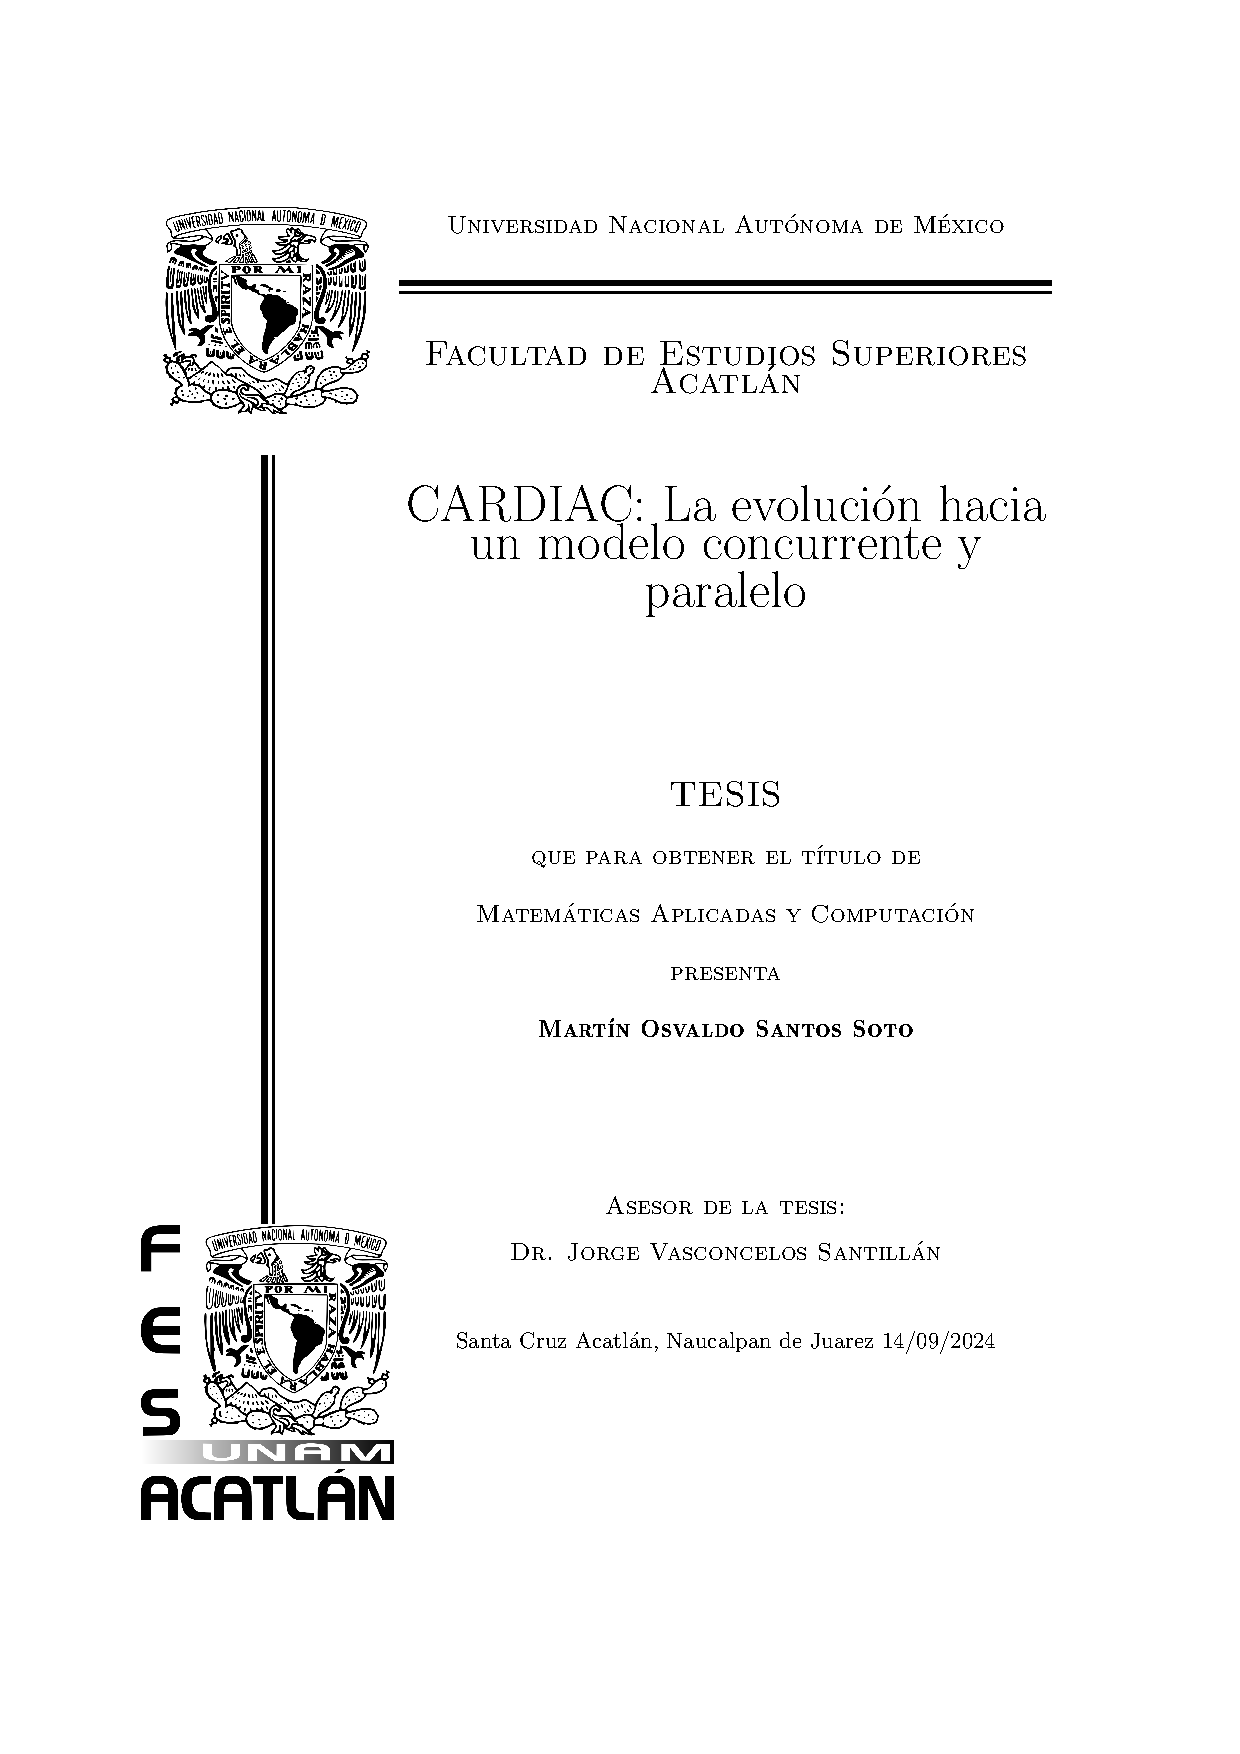
\includepdf{media/cover.pdf}

%---------------------------------
\chapter*{}
\begin{flushright}%
  \emph{``These are fast-moving times, and those who make no effort to understand computers may very well get left behind''}
  
  
  - David W. Hagelbarger, 1968
  %%\thispagestyle{empty}
\end{flushright}

\chapter*{Agradecimientos}
%\spacing{1.5}%\doublespacing

\chapter*{Abstract}

\chapter{Introducción}

	Hoy en día tenemos multitud de aparatos electrónicos que pueden ser llamados computadoras; celulares, laptops, tabletas, relojes inteligentes, y un sin fin más. 
	Estos aparatos pueden ser llamados así siempre que sean  capaces de resolver operaciones aritméticas y lógicas de manera automática, al menos en la definición
	más aceptada que recoge el diccionario de Cambridge(dado que la palabra de origen es anglosajona en este contexto),
	por que sin analizamos más detalladamente el termino ``computadora''  notaremos que el origen de la palabra es anterior a las computadoras
	tal cual las conocemos hoy día, por ejemplo las primeras nociones de ``computadoras''  eran referidas a mujeres de los años 1930 en estados unidos
	que trabajaban en la NASA y realizaban cálculos manuales, por ende podemos deducir que ese termino fue cambiando hasta ser lo que es hoy.
	Si analizamos la historia notaremos que el avance científico en cuanto a maquinas
	que pudieran automatizar tareas que realizaba la humanidad estaban centrados en las calculadoras, había que hacer los cálculos matemáticos menos
	complejos, ya sea con técnicas como los logaritmos y las tablas de multiplicar que se tenían
	para consultar más rápidamente operaciones complejas y repetitivas o con la invención de maquinas que pudieran automatizar calculos, pero con el tiempo el mismo desarrollo de estas maquinas dio paso a algo más,
	a una maquina de propósito general, programable y que ya no solo resolvía operaciones aritméticas, sino que hacía pruebas lógicas y podías
	adaptarla a problemas más particulares, así se fueron formando las ``computadoras'', que como podemos notar son un tipo de evolución de las calculadoras en el sentido de los usos y objetivos
	que tenían al principio. Por ende parece coherente que	de las mujeres que trabajaban haciendo cálculos en la NASA manualmente se les llamase ``computadoras'' por que hacían cálculos manuales
	de forma repetida y que de ahí tomarán el nombre los aparatos más sofisticados que se empezaron a ver en la década de 1940 que resolvían estos problemas y que ahora conocemos con el nombre de ``computadoras''.
	%Sinonimos?
	%%https://www.smithsonianmag.com/science-nature/history-human-computers-180972202/
	
	Para ahondar en está relación de las calculadoras y las computadoras hay que regresar al siglo 19, e ir un poco a los orígenes de la computación,
    más precisamente en el año 1830, con el entusiasta Charles Babbage, que había desarrollado una maquina llamada ``Differential Engine''
	que resolvía ecuaciones matemáticas, una calculadora potente si lo queremos ver desde otra perspectiva. Pero su empeño en los siguientes años 
	se centraría en el diseño y constricción
	de su ``Analytical Engine'', que aunque fue imposible de construir por la tecnología de la época, ya fue pensada como una computadora
	de propósito general, en el sentido que podía hacer cálculos y resolver operaciones lógicas además de que era una maquina que se podía programar,
	cumpliendo así todos los puntos básicos para poder ser considerada como una computadora, lamentablemente no pudo llegar a ver la luz de la mano
	de su creador por las limitantes técnicas de la época, pero dejo un precedente.
	
	En esté sentido podemos ver que las computadoras, o más bien su creación ha llevado mucho tiempo para concretarse en lo que tenemos hoy, que es algo mucho
	más complejo que una calculadora, y aunque sabemos de la complejidad de estos aparatos cuando vemos alguno ¿analizamos como es que funcionan por dentro? ¿como podemos enviar mensajes de texto mientras escuchamos una canción? ¿hay algún programa que ejecuta a los programas que utilizamos? ¿hay un programa que da inicio a todos los procesos de una computadora?
	usualmente la respuesta es ``No'', que no es necesariamente una respuesta mala, en el día a día no podemos detenernos a analizar cada artefacto que tengamos cerca o usemos, a pesar de que sería muy útil saberlo,
	si funciona el aparato es todo lo que necesitamos saber, después de todo hay muchos artefactos o situaciones
	a las cuales prestar atención. Sin embargo, para los profesionales del área de la computación o tecnología en general, así como a aquellos interesados
	por estás tecnologías son preguntas que no pueden faltar. Y es que incluso si tu trabajo es el desarrollo web o
	el diseño de gráficas(que parecieran disciplinas muy lejanas al funcionamiento de un ordenador) entender las razones por las cuales tu computadora o las computadoras para las cuales desarrollas programas pueden hacer cómputos
	en paralelo o tener la potencia que tienen es fundamental para poder optimizar tus desarrollos en la web, los videojuegos que se crean o las gráficas tan detalladas que tenemos en muchos archivos de multimedia; que decir si tu trabajo es la parte del hardware, en ese
	caso debes estar totalmente involucrado con el funcionamiento interno de las computadoras.
	Más aún, considero que al igual que en toda disciplina la historia de la misma o de los artefactos que estudia está debe ser conocida por
	los interesados en la disciplina, pero sobretodo por los profesionales, dado que hay que entender como ha sido la evolución, lo que ha cambiado,
	aquello que a pesar de los años sigue vigente y la razón por la cuál sigue vigente.
	
	
	Centrándonos en el último punto, la historia, es uno de los apartados que a muchas personas les puede parecer tedioso o complicado, 
	por que a pesar de que la historia de las computadoras modernas es corta hablando del tiempo
	de la humanidad, es larga a nivel de la evolución que ha habido en los últimos 80 años, y esto es lo que puede parecer realmente tedioso, sólo hay que ver las diferencias entre
	las computadoras actuales y aquellas que corrían con Windows 98, la diferencia ya es enorme. Ahora si vamos más  a las primeras computadoras personales
	que aún corrían unicamente con línea de comandos y con un paradigma de uso muy diferente al nuestro podemos notar que el cambio ha sido gigante, con todos estos
	cambios uno podría llegar a pensar que una computadora actual ya no tiene prácticamente nada que ver con los ``gigantes de hierro'' de los años 1950, 
	al menos superficialmente se encuentran lejos, pero, internamente de hecho hay muchas similitudes entre estás computadoras. Es más a día de hoy la arquitectura, la estructura
	más general de una computadora actual es exactamente la misma que la de varias de las primeras computadoras, con mejoras en la potencia de
	procesamiento lógicamente, pero con una misma estructura y entender por que esa estructura se ha mantenido vigente hasta nuestros días nos
	llevará a entender lo importante y disruptiva que fue su creación, además de la razón del por que no ha cambiado en todo esté tiempo. Analizando la historia de esa manera, estableciendo conexiones y conociendo que fue lo que continuo
	y aquello que no, ayuda a que esa gigantesca línea del tiempo de las computadoras adquiera otro tono, un tanto menos lleno de datos, que no se quede
	sólo en un montón de fechas y que más bien sea una guía de cambios o sucesos que moldearon el mundo de la computación a lo que hoy conocemos. De está forma podemos conectar los dos puntos que comentaba en el párrafo anterior,
	comprender el funcionamiento de una computadora y conocer la historia de su creación.
	
	 
	Estás preguntas, este análisis principalmente sobre el funcionamiento de las computadoras se dio a lo largo de mi carrera universitaria, y en ese tiempo me di cuenta de lo complejo que podía ser entender
	como funcionaban, después de todo tenía, en principio, la barrera del idioma, dado
	que la lengua franca de la computación es en inglés muchos escritos están en ese idioma, y aunque hay variedad de textos traducidos, otros más,  los más especializados
	o más antiguos es difícil tenerlos en español. Otro tema adicional está en los libros más técnicos, estos 
	manuales
	o libros llenos de teoría acerca del funcionamiento de los ordenadores, la concurrencia, los ordenadores en distribuido, de como funciona el paralelismo, de las necesidades y utilidad del sistema operativo, presentan otro problema además
	del idioma, 
	son realmente difíciles de leer para un estudiante que va empezando en la carrera. Lo curioso es que este problema no es nuevo, ya se habían enfrentado a el no solo muchos
	estudiantes desde la aparición de la computación, sino también muchas instituciones y empresas que querían que más personas aprendieran a usar una computadora,
	aunque cabe aclarar que éste problema cuando empezó a aparecer era un poco distinto por no decir bastante más complejo, y es que esto sucede en los años 60 y 70, cuando se empiezan a popularizar las computadoras, si querías usar una computadora tenías que entender muy bien el como funcionaba por que 
	no había una interfaz gráfica o un sistema operativo que hiciera todas las tareas secundarías por ti, tenías que entender como se movía por dentro la computadora para
	poder programar y resolver tus problemas, además de que tu acceso era muy limitado por lo que no podías perder el tiempo. Es aquí, en este periodo histórico, más precisamente en los años 60, cuando varias compañías e instituciones
	educativas comienzan a lanzar ciertos modelos, manuales y kits para que los estudiantes aprendieran a usar las computadoras
	, algunos básicamente eran un kit de papel con un manual, una ``computadora de papel'' como se les ha llamado, en la cual tu como estudiante
	podías ver como eran las ejecuciones del código que habías escrito, y como eso se materializaba en una respuesta a tu problema inicial. Una de estás fue 
	``Little Man Computer(LMC)'' creada por Stuart Madnick y Jhon Donovan del MIT en los años 60, que con un reducido set de instrucciones permitía a los estudiantes probar la
	ejecución de programas como si estuvieran en una computadora real, otra de mucha relevancia fue su contemporánea CARDIAC(CARDboard Illustrative Aid to Computation) 
	desarrollada por Bell Labs de la mano de David W. Hagelbarger y Saul Fingerman, que es
	muy similar a lo descrito sobre LMC, pero con su propio lenguaje y su propia arquitectura, que incluso llego a ser  más popular
	por el poder de Bell Labs en aquellos tiempos que logro distribuirla en muchas instituciones educativas de estados unidos.
	Lo cual no fue realmente difícil por que en  los años de 1960 
	las computadoras eran ordenadores gigantes y conseguir tiempo para usarlos era realmente difícil, comprarlos directamente imposible para las personas
	comunes, entonces la solución que encontraron para que los estudiantes pudieran practicar fue la creación de estos kits con computadoras de papel, que los
	preparaban  para cuando pudieran usar una computadora ``real''.
	 Hubo otros desarrollos en años siguientes que tuvieron el mismo fin, dado que lo común en los años posteriores y quizá hasta hace algunos años en algunas partes del mundo, fue que acceder a las computadoras reales era o es casi imposible,
	además de que hay más razones por las cuales estos modelos nos pueden ser realmente útiles.

%%link al kit armable
	Eso quizá nos pueda parecer una simple clase de historia de la computación, pero no lo es, CARDIAC sigue siendo muy útil, por que como mencioné, hay más razones por las cuales nos sigue siendo ayudando, de hecho
	funciona para explicar una buena parte del funcionamiento de a las computadoras de una forma sencilla pero a la vez precisa, yo experimente el uso de CARDIAC en una clase de programación paralela y concurrente en la 
	cual esté modelo
	fue fundamental para entender los conceptos básicos de los que parte la computación. También hay que ser consientes que con un modelo cómo CARDIAC no te vas a volver un experto en 
	el funcionamiento de las computadoras,
	pero el punto es entender de una forma clara su estructura de modo que tengas las bases para entonces ser capaz de leer uno de esos manuales llenos de teoría sobre sistemas
	operativos y arquitectura de computadoras con muchísimos conceptos técnicos, los cuales si no tienes cierto conocimiento de base terminan siendo muy complicados de leer y entender.
	
	Aún con todas estás ventajas de CARDIAC, las limitaciones son evidentes, fue construida en el año 1968, no es apta para la concurrencia ni el paralelismo, o 
	incluso un computo distribuido, por esa razón muchas personas que están en el mundo de la computación en los años posteriores han seguido haciendo
	modelos similares como MARIE(Machine Architecture that is Really Intuitive and Easy) o directamente evoluciones de ella como TIMBA(Terrible Imbecile Machine for Boring 
	Algorithms), algunos más técnicos que otros, y aunque la mayoría están en inglés hay varios proyectos en español. 
	Al adentrarme más en estos modelos me di cuenta que un buen modelo que explicará el funcionamiento de computadoras más recientes en los componentes de su arquitectura se volvían más técnicos, como el 
	desarrollo mexicano de \textit{8 bit a complete Design}, 
	que es un gran trabajo, pero que termina usando bastantes conceptos que requieren ciertas bases de conocimiento y aquellos que no son tan técnicos caen un poco en ser bastante similares a CARDIAC, lo cual no 
	es malo, e incluso tiene muchas ventajas que mejoran algunas lagunas de CARDIAC, pero hay otras más que no intentan solucionar por diversas razones. Es en esté punto en el que decidí empezar este
	proyecto de investigación para explicar como funcionan las computadoras de una forma simple y didáctica para aquellos estudiantes que van empezando la carrera
	como forma de contestar esas preguntas tan generales que plantee al principio,
	tomando como base el  desarrollo de CARDIAC y llevándola unos pasos más allá en nivel de arquitectura para que sea capaz de explicar
	la computación concurrente y paralela, así como entender la necesidad de un sistema operativo en maquinas más complejas sin dejar de lado la simplicidad que la 
	caracteriza.
	Con un enfoque particular que lleve al lector a ver las necesidades de hardware y software que hacen evolucionar a CARDIAC,
	de forma que se entienda la razón de la evolución de las computadoras en varios ámbitos fundamentales, y en ese mismo sentido situarse en la línea
	temporal en que surgieron esos cambios para entender su contexto histórico y como lo mencione antes, entender por que hay características  que siguen vigentes
	80 años después en los ordenadores y otras 	que no.
	
	
	Más allá del recorrido en la construcción y diseño de modelos ``evolucionados'' de CARDIAC para computación paralela y concurrente el texto se verá acompañado,
	tal como la clásica CARDIAC distribuida por Bell Labs, con un ``kit'' que incluye un programa que contendrá tres maquinas virtuales, uno para cada
	modelo de CARDIAC, con la diferencia de que estas maquinas virtuales ya no serán en papel, sino interfaces gráficas para uso en computadoras de escritorio con la idea de que sea fácil para el estudiante
	entender la teoría y practicarla, poder ver como se van ejecutando los programás que ya en una versión paralela o concurrente sería un poco más difícil de ver con una computadora de papel dada la cantidad de información que se tiene que almacenar.
	
	%%Le falta algo al cierre%%



\tableofcontents
\listoffigures

\mainmatter

\chapter{Teoría e historia de la computación} %


\section{Las computadoras en la historia}
	\subsection{Primeros autómatas}
	% Breve historia de como se fue desarrollando la computación desde los inicios hasta llegar a automatas(1950)
	\subsection{Primeras computadoras}
	%1950-1968
	\subsection{Nacimiento de CARDIAC}
	%El como nace el modelo para dar claridad a los trabajadores de ATT
	\subsection{Primeros Sistemas Operativos}
	
	\subsection{Indicios de concurrencia y paralelismo}
	
	\subsection{Actualidad de las computadoras}
   
\section{Funcionamiento de las computadoras}   
	\subsection{Arquitectura Von Neumann}   

	\subsection{Sistema Operativo}   	
   	
	\subsection{Modelo concurrente}

	\subsection{Modelo paralelo}


\chapter{CARDIAC y su evolución}  %
	\section{Operaciones concurrentes}
	
		\subsection{Necesidad de un sistema operativo}
		
		\subsection{Mejoras necesarias en el Hardware}
		
		\subsection{Creación de una arquitectura concurrente}
	
	 \section{Evolución hacia el paralelismo}
	 
	 	\subsection{Hardware y sus necesidades}
	 	
	 	\subsection{Arquitectura paralela E-CARDIAC PAR}


\chapter{Conclusiones}

%\bibliographystyle{humannat}
%\bibliography{references}

%\backmatter%@sglvgdor


\end{document}

